\section{Linee guida per gli esercizi}
\subsection{Impostazione del problem}
\begin{itemize}
    \item Leggere bene il testo del problema.
    \item Effettuare una schematizzazione del problema: identificare il tipo di sistema, il suo
    contorno, la sostanza evolvente nel sistema, gli scambi di massa, calore e lavoro con
    l’ambiente e la loro direzione.
    \item Scrivere i dati forniti dal testo del problema, e le incognite da ricavare per risolverlo.
    Convertire i dati in unità di misura congruenti e conformi al Sistema Internazionale.
    \item Se avvengono trasformazioni termodinamiche, rappresentarle qualitativamente su un
    diagramma opportuno.    
\end{itemize}
\subsection{Soluzione del problema}
\begin{itemize}
    \item Scrivere i bilanci di massa, energia ed entropia per il volume di controllo considerato.
    Elencare le ipotesi applicabili al sistema (riguardo la natura del contorno del sistema, delle
    trasformazioni che avvengono al suo interno, delle sostanze delle quali è composto), e
    semplificare i bilanci di conseguenza, ponendo attenzione alle convenzioni di segno.
    \item Scrivere la soluzione analitica del problema.
    \item Risolvere il problema numericamente. Si raccomanda di scrivere sempre le unità di misura
    delle grandezze calcolate e di fare l’analisi dimensionale delle equazioni scritte.
    \item Fare sempre caso alla ragionevolezza dei risultati  
\end{itemize}
\subsection{Unità di misura}
\begin{center}
    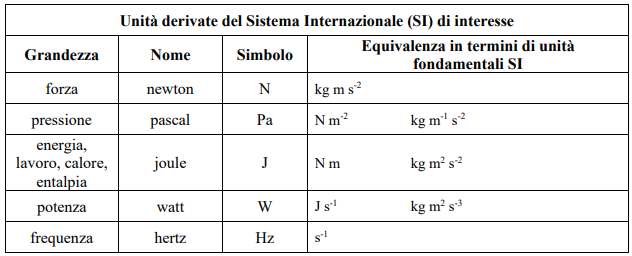
\includegraphics[height=5cm]{../L01/img10.PNG}
\end{center}
\begin{center}
    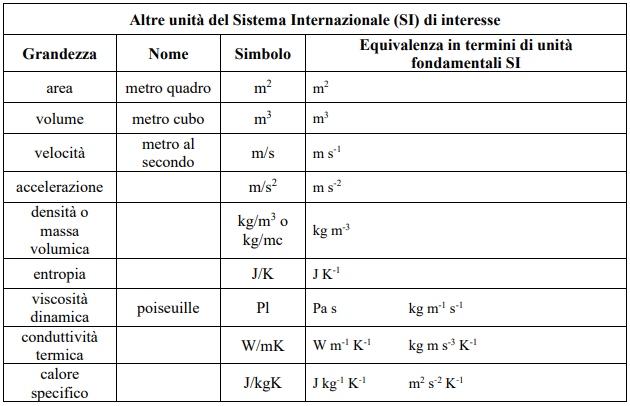
\includegraphics[height=7cm]{../L01/img11.PNG}
\end{center}
\begin{center}
    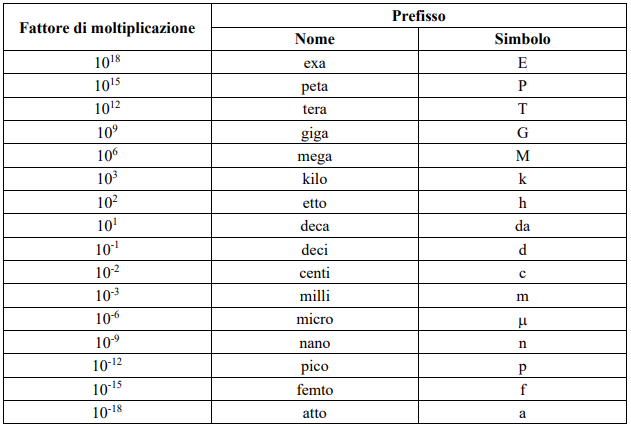
\includegraphics[height=5cm]{../L01/img12.PNG}
\end{center}
\begin{center}
    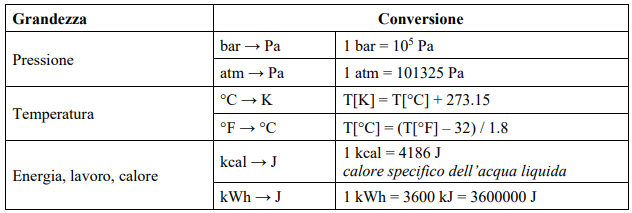
\includegraphics[height=5cm]{../L01/img13.PNG}
\end{center}